\section{Brain Correspondence}
\label{sec:brain_correspondence}


\begin{figure}[htbp]
\centering
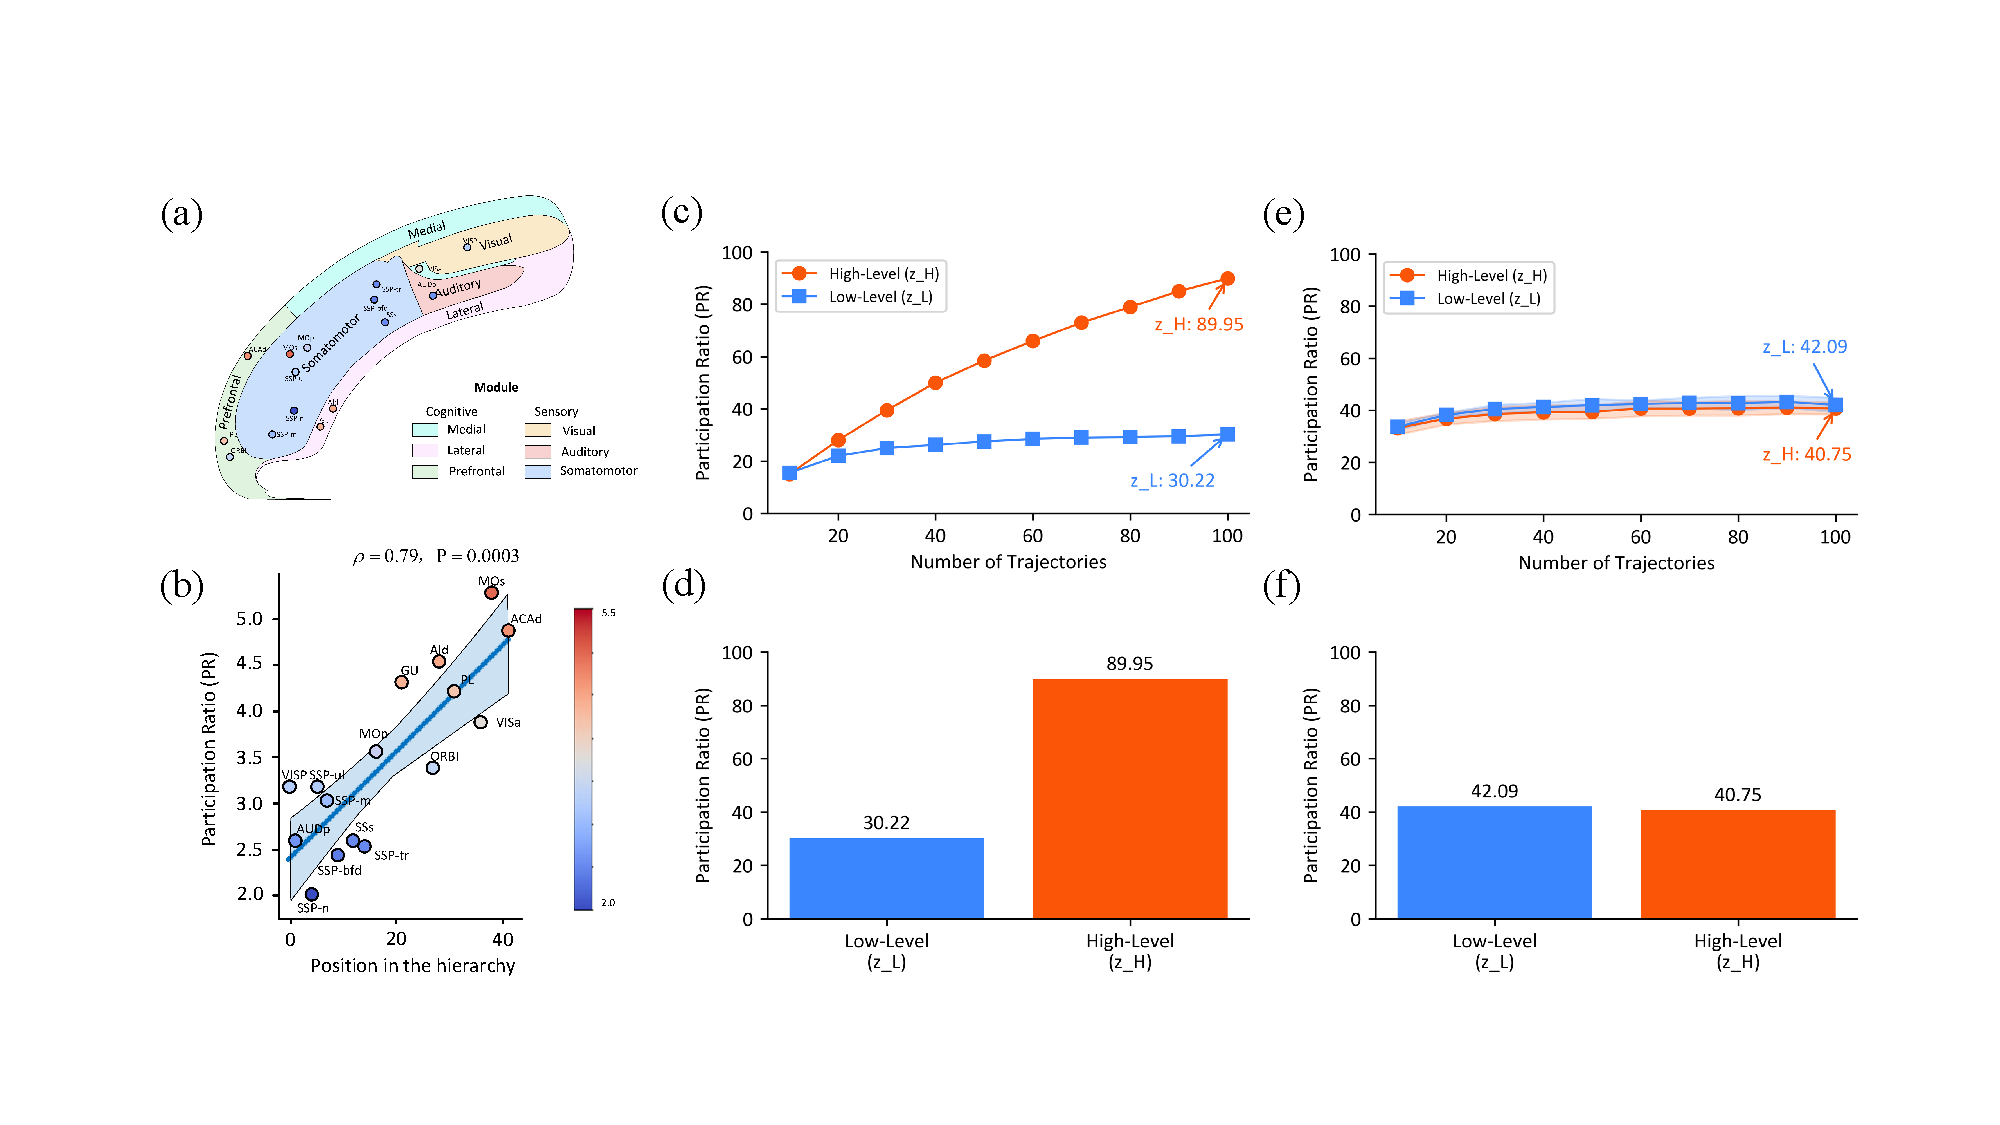
\includegraphics[width=0.95\linewidth]{figures/analysis/hierarchical_dimensionality.pdf}
\caption{
    \textbf{Hierarchical Dimensionality Organization in the HRM and Mouse Cortex.}
    (a,b) are adapted from~\citet{posani2025rarely}.
    (a) Anatomical illustration of mouse cortical areas, color-coded by functional modules.
    (b) Correlation between Participation Ratio (PR), a measure of effective neural dimensionality, and hierarchical position across different mouse cortical areas. Higher positions in the hierarchy (e.g., MOs, ACAd) exhibit significantly higher PR values compared to lower sensory areas (e.g., SSp-n), with a Spearman correlation coefficient of $\rho$ = 0.79 (P = 0.0003).
    (c,d) \textbf{Trained HRM.}
    (c) PR scaling of the trained HRM with task diversity. The dimensionality of the high-level module ($z_H$) scales with the number of unique tasks (trajectories) included in the analysis, indicating an adaptive expansion of its representational capacity. In contrast, the low-level module's ($z_L$) dimensionality remains stable.
    (d) PR values for the low-level ($z_L$, PR = 30.22) and high-level ($z_H$, PR = 89.95) modules of the \emph{trained} HRM, computed from neural activity during 100 unique Sudoku-solving trajectories. A clear dimensionality hierarchy is observed, with the high-level module operating in a substantially higher-dimensional space.
    (e,f) \textbf{Analysis of Untrained Network.} To verify that the dimensionality hierarchy is an emergent property of training, the same analyses were performed on an \emph{untrained} HRM with random weights.
    (e) In contrast to the trained model's scaling in (c), the dimensionality of both modules in the untrained model remains low and stable, failing to scale with the number of tasks.
    (f) Similarly, contrasting with the clear separation in (d), the PR values for the untrained model's modules ($z_L$, PR = 42.09; $z_H$, PR = 40.75) are low and nearly identical, showing no evidence of hierarchical separation. This confirms that the observed hierarchical organization of dimensionality is a learned property that emerges through training, not an artifact of the model's architecture.
}
\label{fig:hierarchical_dimensionality}
\end{figure}

A key principle from systems neuroscience is that a brain region's functional repertoire—its ability to handle diverse and complex tasks—is closely linked to the dimensionality of its neural representations~\citep{rigotti2013importance, mante2013context}. Higher-order cortical areas, responsible for complex reasoning and decision-making, must handle a wide variety of tasks, demanding more flexible and context-dependent processing~\citep{miller2001integrative}. In dynamical systems, this flexibility is often realized through higher-dimensional state-space trajectories, which allow for a richer repertoire of potential computations~\citep{maass2002realtime}. This principle gives rise to an observable \emph{dimensionality hierarchy}, where a region's position in the processing hierarchy correlates with its \emph{effective dimensionality}. To quantify this phenomenon, we can examine the Participation Ratio (PR), which serves as a standard measure of the effective dimensionality of a high-dimensional representation~\citep{altan2021estimating}. The PR is calculated using the formula 
\begin{equation*}
    \text{PR} = \frac{(\sum_{i} \lambda_i)^2}{\sum_{i} \lambda_i^2} \,,
\end{equation*}
where $\{\lambda_i\}$ are the eigenvalues of the covariance matrix of neural trajectories.
Intuitively, a higher PR value signifies that variance is distributed more evenly across many dimensions, corresponding to a higher-dimensional representation. Conversely, a lower PR value indicates that variance is concentrated in only a few principal components, reflecting a more compact, lower-dimensional structure.

The dimensionality hierarchy can be observed, for example, in the mouse cortex, where the PR of population activity increases monotonically from low-level sensory areas to high-level associative areas, supporting this link between dimensionality and functional complexity~\citep{posani2025rarely} (\Cref{fig:hierarchical_dimensionality} (a,b)).

We evaluated whether HRM reproduces this neuroscientific principle by calculating the PR for both recurrent modules after training on the \textit{Sudoku-Extreme Full} dataset. The PR computation used the covariance matrix derived from neural states gathered across multiple Sudoku-solving trajectories. The results show a striking parallel to the biological findings. The low-level module's state ($z_L$) occupies a relatively small subspace with a participation ratio of 30.22, whereas the high-level module's state ($z_H$) operates in a substantially larger subspace with a participation ratio of 89.95, as shown in \Cref{fig:hierarchical_dimensionality}(c).
Furthermore, \Cref{fig:hierarchical_dimensionality}(d) shows that increasing the number of unique tasks (trajectories) from 10 to 100 causes $z_H$ dimensionality to scale up accordingly, while $z_L$ dimensionality remains stable. These results suggest an \emph{emergent} separation of representational capacity between the modules that parallels their functional roles.

To confirm that this hierarchical organization is an emergent property of training, and not an artifact of the network's architecture, we performed a control analysis using an identical but untrained network with random weights.

We initialized an identical HRM architecture with random weights and, without any training, measured the PR of its modules as the network processed the same task-specific inputs given to the trained model.

The results, shown in
\Cref{fig:hierarchical_dimensionality}(e,f), reveal a stark contrast: the high-level and
low-level modules of the untrained network exhibit no hierarchical separation, with their PR values
remaining low and nearly indistinguishable from each other. This control analysis validates that
the dimensionality hierarchy is an \emph{emergent property} that arises as the model
learns to perform complex reasoning.

The high-to-low PR ratio in HRM ($z_H/z_L \approx 2.98$) closely matches that measured in the mouse
cortex ($\approx 2.25$). In contrast, conventional deep networks often exhibit \emph{neural collapse},
where last-layer features
converge to a low-dimensional
subspace~\citep{papyan2020prevalence,fang2021layerpeeled,zhu2021geometric}.
HRM therefore departs from the collapse pattern and instead fosters a high-dimensional representation in its higher module. This is significant because such representations are considered crucial for cognitive flexibility and are a hallmark of higher-order brain regions like the prefrontal cortex (PFC), which is central to complex reasoning.

This structural parallel suggests the model has discovered a fundamental organizational principle. By learning to partition its representations into a high-capacity, high-dimensional subspace ($z_H$) and a more specialized, low-dimensional one ($z_L$), HRM autonomously discovers an organizational principle that is thought to be fundamental for achieving robust and flexible reasoning in biological systems. This provides a potential mechanistic explanation for the model's success on complex, long-horizon tasks that are intractable for models lacking such a differentiated internal structure. We emphasize, however, that this evidence is correlational. While a causal link could be tested via intervention (e.g., by constraining the H-module's dimensionality), such methods are difficult to interpret in deep learning due to potential confounding effects on the training process itself. Thus, the causal necessity of this emergent hierarchy remains an important question for future investigation.
